
%\subsubsection{International Patent Classification code}
%In 1971, the Strasbourg Agreement established the International Patent Classification (IPC) under the World Intellectual Property Organization (WIPO), which divides technology into eight discrete Sections. The goal of this
%Agreement was to overcome the difficulties caused by using diverse national patent classification systems.~\citep{harris2010comparison}
%
%A patent is assigned to one or more of the 71,000 IPC codes that 
%indicate the related technical field or fields the patent covers. 
%These codes are arranged in a hierarchical, tree-like structure with 
%five distinct components. Fig. \ref{fig:ipcexample} illustrates the components of an IPC classification.
%
%The highest hierarchical level contains the eight sections of the IPC corresponding
%to very broad technical fields, labeled A through H. For example, Section C deals
%with``Chemistry and Metallurgy''. Sections are subdivided into classes. The eighth edition of the IPC contains 120
%classes. Class C07, for example, deals with ``Organic Chemistry''. Classes are further subdivided into more than 600 subclasses. Subclass C07C, for example, deals with ``Acyclic or Carbocyclic Compounds''. Subclasses are then further divided into main groups and subgroups. Main group symbols end with ``/00''. Ten percent of all IPC groups are main
%groups. For example, main group C07C 35/00 deals with ``Compounds having at
%least one hydroxy or O-metal group bound to a carbon atom of a ring other than
%a six-membered aromatic ring''. In some versions of the IPC, a series of numbers will follow the subgroup, reflecting
%the enactment date of the IPC version. `20060101' following the Subgroup
%indicates a date of January 1, 2006, which is the date that the eighth version of
%the IPC took effect. 
%%%%%%%%%%%%%%%%%%%%%%%%%%%%%%%%%%%%%%%%%%%%%%%%%%%%%%%%%%%%%%%%%%%%%%%%%%%%%%%%%%
%\begin{figure}[t!]
%   \centering
%   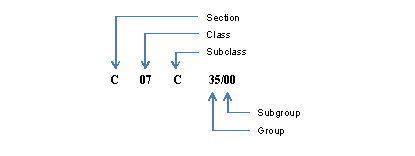
\includegraphics[width=0.70\textwidth,height=35mm]{figs/IPCexample.jpg}
%   \caption{An example illustrating the components of an International Patent Classification code.}   
%   \label{fig:ipcexample} 
%\end{figure}
%%%%%%%%%%%%%%%%%%%%%%%%%%%%%%%%%%%%%%%%%%%%%%%%%%%%%%%%%%%%%%%%%%%%%%%%%%%%%%%%%%
%\subsubsection{IPC Classification as a Filter}
As we mentioned in section~\ref{sec:settings}, International Patent Classification (IPC) codes (section~\ref{StructureofPatents}) 
assigned to topics to filter the search results by constraining them to have common IPC codes with the patent topic.
In this section, we investigate the errors related to classification code mismatch between topics and relevant documents for three different level of hierarchy. 
 
%\subsubsection{Applying 4-digit IPC code for filtering}
%\label{subsec: 4-digit}
\paragraph{(I) Applying three first IPC components for filtering}
\ \\
In our experimental settings, we filtered the search results using three first symbols of IPC code including Section, Class, and Subclass. Using IPC filter prevents retrieval of relevant documents which do not share any IPC code with patent query. 

Our experiments show that   
around 19\% of not-retrieved relevant patents do not share any IPC code with the patent query, but the majority of them have query main IPC code, and about 21\% share, at least, one of the query further IPC codes (Figure~\ref{fig:ipcoverlap_a}). 
%%%%%%%%%%%%%%%%%%%%%%%%%%%%%%%%%%%%%%%%%%%%%%%%%%%%%%%%%%%%%%%%%%%%%%%%%%%%%%%%%
%\begin{figure}[t!]
%   \centering
%   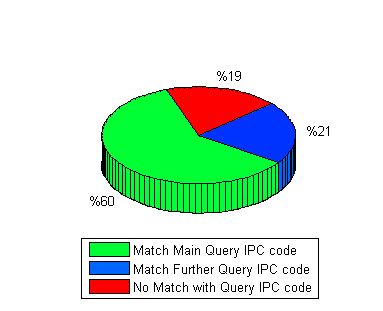
\includegraphics[width=0.60\textwidth,height=69mm]{figs/ipcOverlap-FNs.png}
%   \caption{Classification code overlap between the query and non-relevant retrieved patents (False Negative (FN) patents).}   
%   \label{fig:fnipcoverlap} 
%\end{figure}
%%%%%%%%%%%%%%%%%%%%%%%%%%%%%%%%%%%%%%%%%%%%%%%%%%%%%%%%%%%%%%%%%%%%%%%%%%%%%%%%%
%%%%%%%%%%%%%%%%%%%%%%%%%%%%%%%%%%%%%%%%%%%%%%%%%%%%%%%%%%%%%%
\begin{figure}[t!]
\begin{centering}
\subfigure[non-relevant retrieved patents (False Negative (FN) patents)\label{fig:ipcoverlap_a}]{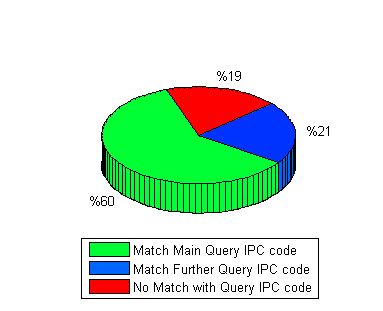
\includegraphics[width=6.5cm]{figs/ipcOverlap-FNs.png}} 
\hspace*{0.5cm}  \subfigure[relevant retrieved patents (True Positive (TP) patents)\label{fig:ipcoverlap_b}]{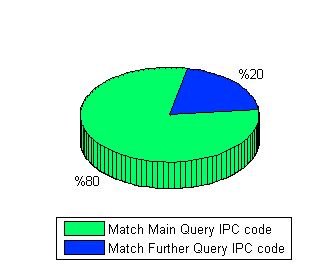
\includegraphics[width=6.5cm]{figs/ipcOverlap-TPs.png}} 

\par\end{centering} 
\protect\caption{Classification code overlap between the query and non-relevant retrieved patents (False Negative (FN) patents).}
\label{fig:ipcoverlap}
\end{figure}
%%%%%%%%%%%%%%%%%%%%%%%%%%%%%%%%%%%%%%%%%%%%%%%%%%%%%%%%%%%%%%
On the other hand, as it has been shown in Figure \ref{fig:ipcoverlap_b}, 80\% of TP patents have an overlap with the main IPC code of the query and 20\% with, at least, one of the query further IPC codes. 
%So, we can conclude that 19\% of errors can be due to IPC filtering if we assume that they have enough term overlap with the query.  
%%%%%%%%%%%%%%%%%%%%%%%%%%%%%%%%%%%%%%%%%%%%%%%%%%%%%%%%%%%%%%%%%%%%%%%%%%%%%%%%%
%\begin{figure}[t!]
%   \centering
%   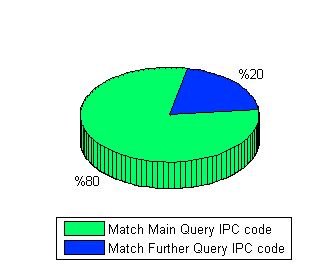
\includegraphics[width=0.55\textwidth,height=60mm]{figs/ipcOverlap-TPs.png}
%   \caption{Classification code overlap between the query and relevant retrieved patents (True Positive (TP) patents).}   
%   \label{fig:tpipcoverlap} 
%\end{figure}
%%%%%%%%%%%%%%%%%%%%%%%%%%%%%%%%%%%%%%%%%%%%%%%%%%%%%%%%%%%%%%%%%%%%%%%%%%%%%%%%%

We can not retrieve around 19\% of relevant patents as the result of applying IPC filter, however, we still keep using the filter in our experiments for two main reasons: 
\begin{enumerate}
\item CLEF-IP 2010 collection contains 2.6 million patent documents. If we set the filter: \textit{off}, it will be time consuming to match the query to the whole collection. However, by applying the filter, this process will be done faster and instead of the whole collection, matching process is done on the portion of the collection which share an IPC code with the patent query. Since less than 19\% of errors are due to classification mismatch, we continue our analysis by keeping the filter: \textit{on} because the matching process is computationally much faster compared to what we lose by applying the IPC filter. The computational time is critical in patent prior art search as the query is the Description of the the patent query, which contains thousands of words.   
\item Precision in the top k=100 drops significantly when ranking the whole collection versus the portion that have shared classification code with the query.  
\end{enumerate}

To justify the first reason, in the following experiment, we calculate the number of documents which have at least one of the query IPC code. In average, this number is $ 36254 $, which indicates for each query, the system just needs to look into $ 36254 $ documents in average instead of the entire collection that contains 2.6 million patent documents. Therefore, we will computationally save lots of time if we apply the IPC filter.  
%%%%%%%%%%%%%%%%%%%%%%%%%%%%%%%%%%%%%%%%%%%%%%%%%%%%%%%%%%%%%%%%%%%%%%%%%%%%%%%%%
\begin{figure}[t!]
   \centering
   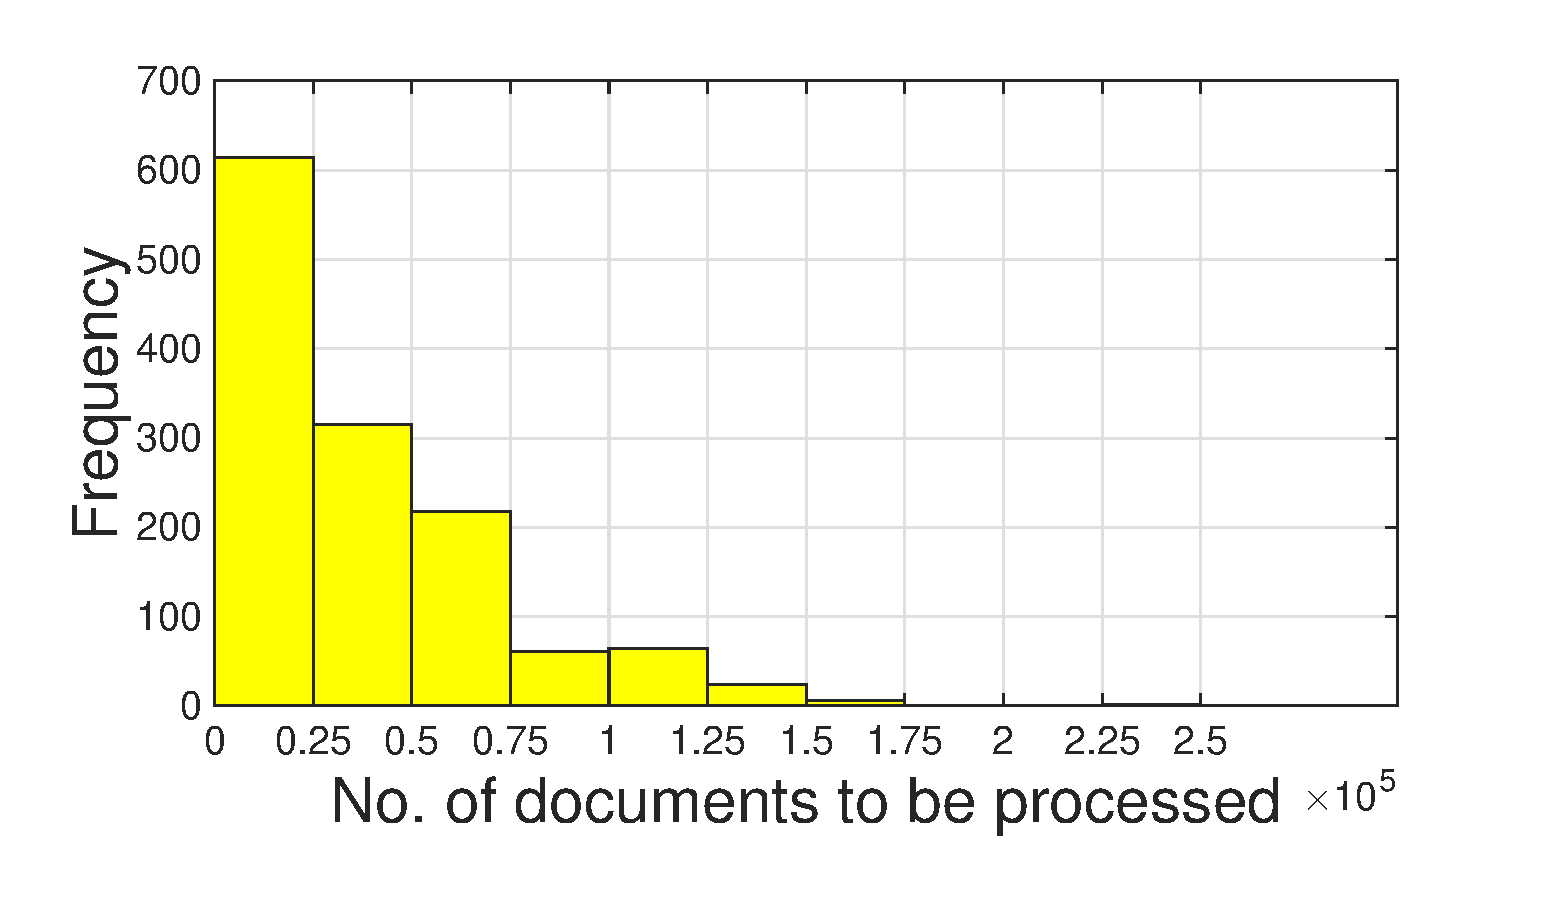
\includegraphics[width=0.70\textwidth,height=55mm]{figs/filter1}
   \caption{The distribution of the number of patents should be ranked for each query over all test topics (1303), after applying the IPC filter: Type I.
In average, the matching process for each query is done over $ 36254 $ documents instead of the whole collection (2.6 million documents) which dramatically reduce the computational time.}   
   \label{fig:ipcfilter-histo} 
\end{figure}
%%%%%%%%%%%%%%%%%%%%%%%%%%%%%%%%%%%%%%%%%%%%%%%%%%%%%%%%%%%%%%%%%%%%%%%%%%%%%%%%%
%\FloatBarrier 
%\noindent

Figure~\ref{fig:ipcfilter-histo} shows the distribution of documents that should be processed for each query after applying IPC filter. 
It illustrates that for the majority of queries the matching process should be only done over $25000$ documents. 
In trade off between losing 19\% of relevant patents and making the ranking process faster, we chose the faster computation. The histogram falls down by increasing the number of documents that should be processed; This means that the majority of queries need to do matching process with less documents. 
%\vspace{-1cm}
%\subsubsection{Applying First two IPC code components for filtering}
%\label{subsec: Firsttwocomponents}
\paragraph{(II) Applying first two IPC code components for filtering}
%\textbf{(B) Filter: First two components of the IPC code}
\ \\
We hypothesize that the errors will be reduced if we broaden the filter by selecting two first components of the query IPC, namely, Section, and Class (e.g., C07).

The results has been illustrated in Figure~\ref{fig:ipc1stTwoElements}. Figure~\ref{fig:ipc1stTwoElements_a} shows that we can reduce the errors related to filtering from 19\% to 13\% by omitting the subclass component. However, the number of documents that should be ranked increases from $ 36254 $ to $ 99754 $ in average. As it can be seen in Figure~\ref{fig:ipc1stTwoElements_b}, the distribution of the number of documents that should be compared in matching process does not follow the falling trend as filtering with three first components. We conclude that this kind of filter is not appropriate since we only reduce the error by 6\% whereas the average number of documents, which should be processed, triples.    
%%%%%%%%%%%%%%%%%%%%%%%%%%%%%%%%%%%%%%%%%%%%%%%%%%%%%%%%%%%%%%%%%%%%%%%%%%%%%%%%%
%\begin{figure}[t!]
%   \centering
%   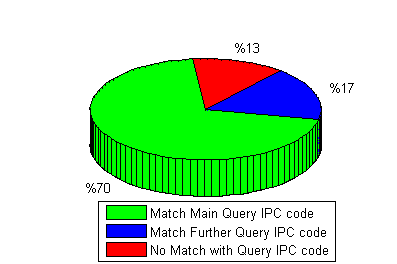
\includegraphics[width=0.55\textwidth,height=60mm]{figs/ipc1stTwoElements.png}
%   \caption{Filter: The first two components (Section and Class).}   
%   \label{fig:ipc1stTwoElements} 
%\end{figure}
%%%%%%%%%%%%%%%%%%%%%%%%%%%%%%%%%%%%%%%%%%%%%%%%%%%%%%%%%%%%%%%%%%%%%%%%%%%%%%%%%
%%%%%%%%%%%%%%%%%%%%%%%%%%%%%%%%%%%%%%%%%%%%%%%%%%%%%%%%%%%%%%
\begin{figure}[t!]
\begin{centering}
\subfigure[The portion of patents in the collection which are matched with the query IPC code. \label{fig:ipc1stTwoElements_a}]{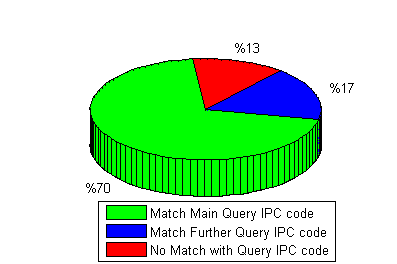
\includegraphics[width=6.5cm, height=5cm]{figs/ipc1stTwoElements.png}} 
\\[1ex]%
\subfigure[The distribution of the number of patents should be ranked for each query over all test queries (1303).
In average, the matching process for each query is done over $ 99754 $ documents instead of the whole collection (2.6 million documents), which dramatically reduce the computational time.\label{fig:ipc1stTwoElements_b}]{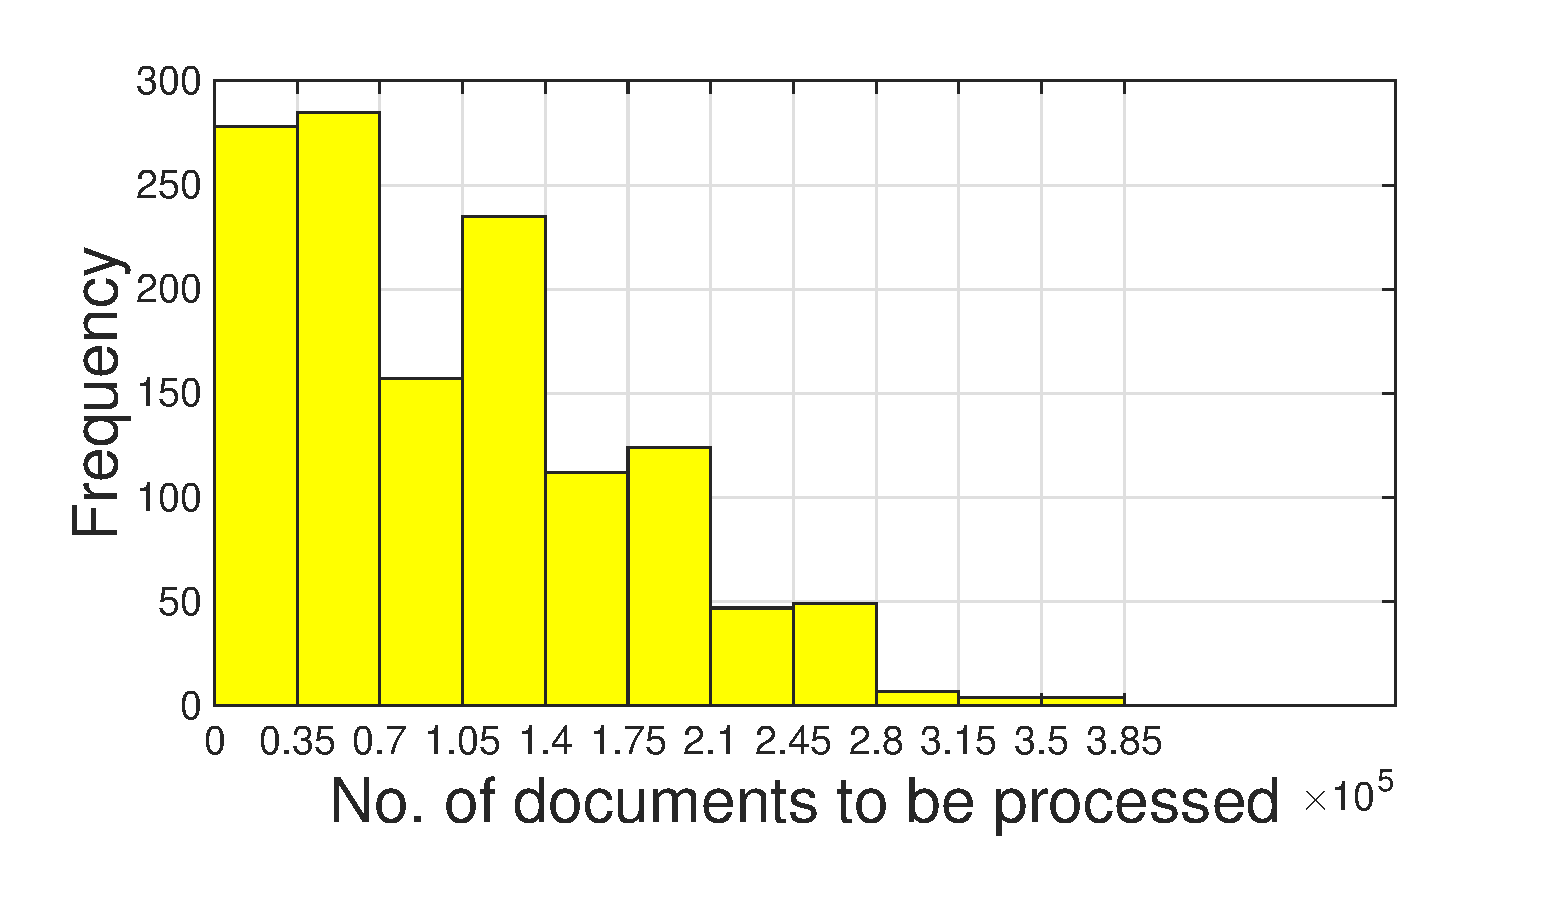
\includegraphics[width=9.5cm, height=6cm]{figs/filter2}} 

\par\end{centering} 
\protect\caption{Applying first two IPC code components (Section and Class) for filtering}
\label{fig:ipc1stTwoElements}
\end{figure}
%%%%%%%%%%%%%%%%%%%%%%%%%%%%%%%%%%%%%%%%%%%%%%%%%%%%%%%%%%%%%%
%\begin{figure}[htpb]
%\centering
%\begin{subfigure}[htpb]{.5\linewidth}
%\centering
%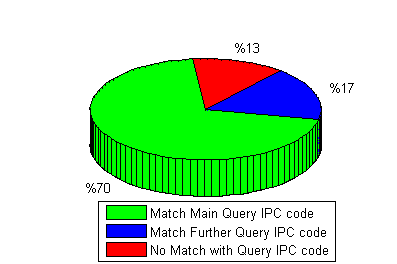
\includegraphics[width=1\textwidth,height=55mm]{figs/ipc1stTwoElements.png}
%\caption{Filter: The first two components (Section and Class)}
%\label{fig:ipc1stTwoElements}
%\end{subfigure}%\\[1ex]%
%\begin{subfigure}[htpb]{.5\linewidth}
%\centering
%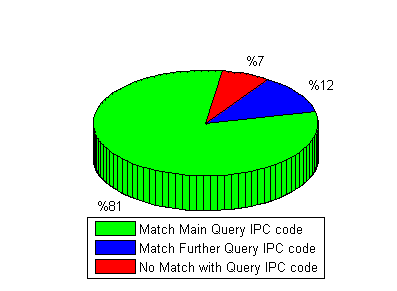
\includegraphics[width=1\textwidth,height=55mm]{figs/ipc1stElement.png}
%\caption{Filter: Only the first component (Section)}
%\label{fig:ipc1stElement}
%\end{subfigure}
%\caption{IPC classification overlap between the query and the FN patents after making the filter broader.}
%\label{fig:restrictedipc}
%\end{figure}
%\FloatBarrier
%%%%%%%%%%%%%%%%%%%%%%%%%%%%%%%%%%%%%%%%%%%%%%%%%%%%%%%%%%%%%%%%%%%%%%%%%%%%%%%%%
%\begin{figure}[t!]
%   \centering
%   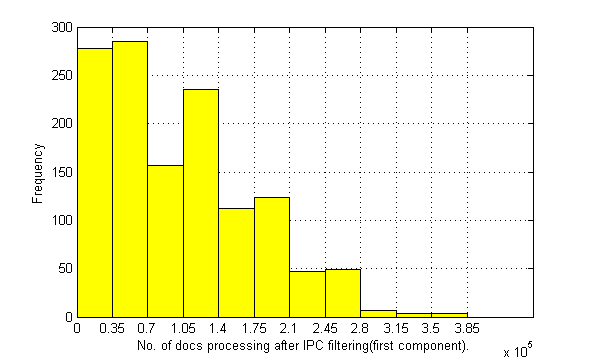
\includegraphics[width=0.70\textwidth,height=68mm]{figs/firstTwoIpcFilter-histo.png}
%   \caption{The distribution of the number of patents should be ranked for each query over all test queries (1303).
%In average, the matching process for each query is done over `$ 99754 $' documents instead of the whole collection (2.6 million documents) which reduce the computational time dramatically.}   
%   \label{fig:firstTwoIpcFilter-histo} 
%\end{figure}
%%%%%%%%%%%%%%%%%%%%%%%%%%%%%%%%%%%%%%%%%%%%%%%%%%%%%%%%%%%%%%%%%%%%%%%%%%%%%%%%%
%\FloatBarrier 
%\vspace{-5em}
%\noindent
%\subsubsection{Applying First two IPC code components for filtering}
%\label{subsec: Firsttwocomponents}
\paragraph{(III) Applying the first IPC code component for filtering}
%\textbf{(C) Filter: First component of the IPC code}
\ \\
We can even make the filter more general by choosing only the first component, namely, Section (e.g., C), corresponding to very general technical fields. 
%%%%%%%%%%%%%%%%%%%%%%%%%%%%%%%%%%%%%%%%%%%%%%%%%%%%%%%%%%%%%%
\begin{figure}[t!]
\begin{centering}
\subfigure[The portion of patents in the collection which are matched with the query IPC code. Filter: The first two components \label{fig:ipc1stElements_a}]{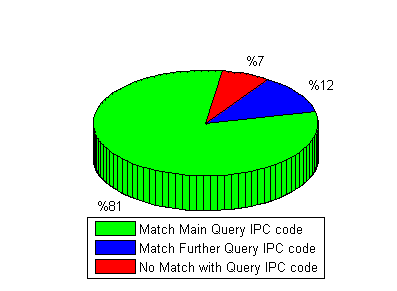
\includegraphics[width=6.5cm, height=5cm]{figs/ipc1stElement.png}} 
\\[1ex]%
\subfigure[The distribution of the number of patents should be processed for each query after applying the IPC filter.
In average, the matching process for each query is done over $ 415828 $ documents instead of the whole collection (2.6 million documents). This number is much higher than using more restricted filters, so it is not computationally efficient.\label{fig:ipc1stElements_b}]{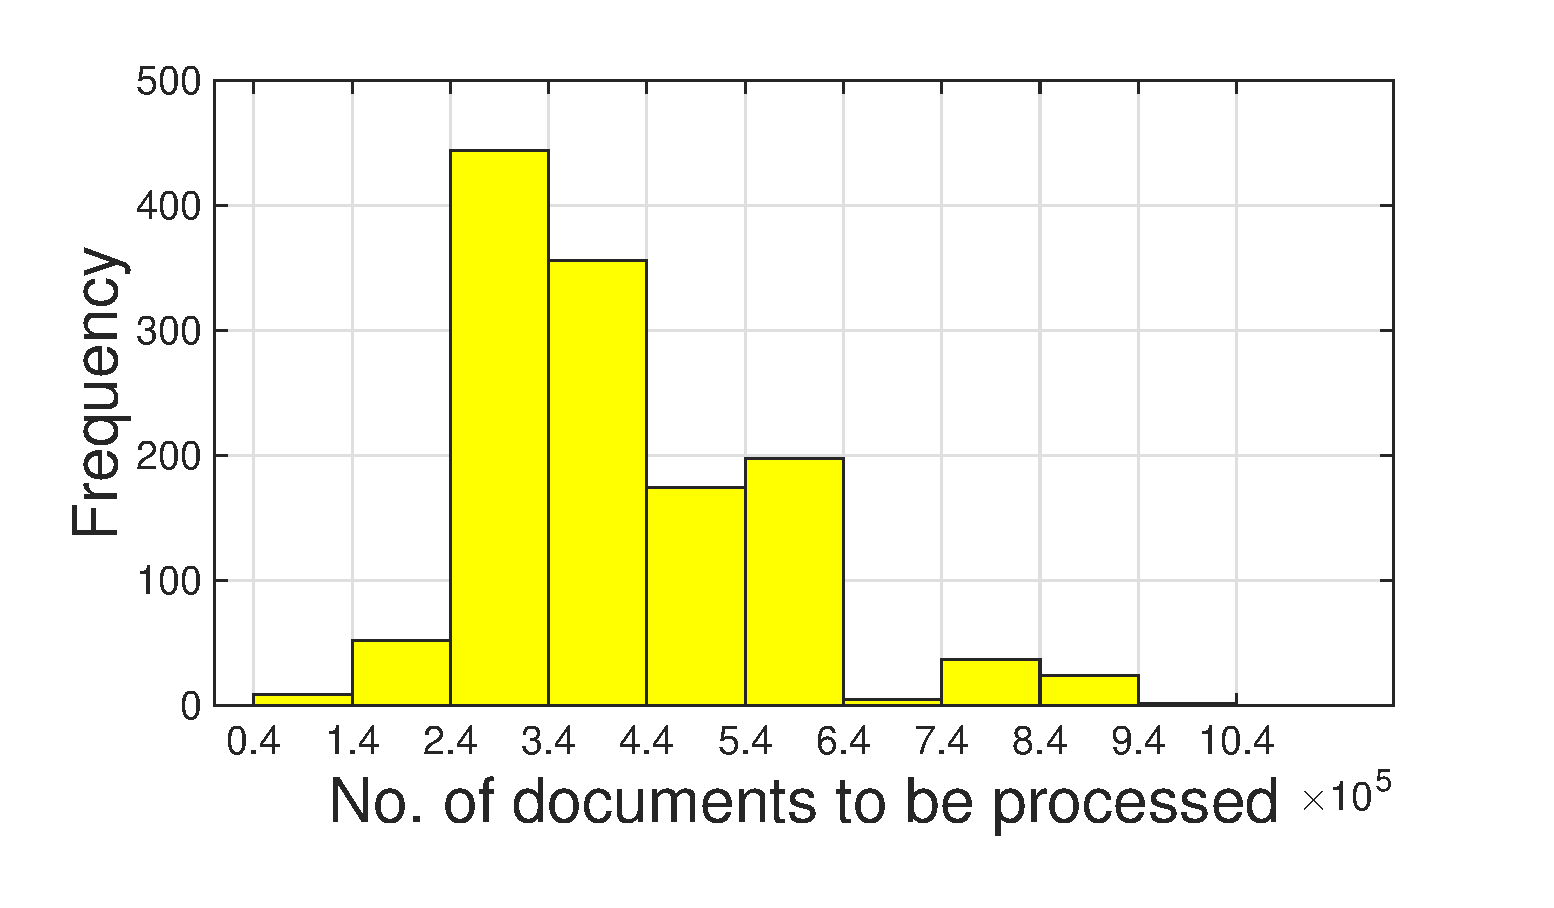
\includegraphics[width=9.5cm , height=6cm]{figs/filter3}} 

\par\end{centering} 
\protect\caption{Applying the first IPC code component for filtering (Section)}
\label{fig:ipc1stElements}
\end{figure}
%%%%%%%%%%%%%%%%%%%%%%%%%%%%%%%%%%%%%%%%%%%%%%%%%%%%%%%%%%%%%%
%%%%%%%%%%%%%%%%%%%%%%%%%%%%%%%%%%%%%%%%%%%%%%%%%%%%%%%%%%%%%%%%%%%%%%%%%%%%%%%%%
%\begin{figure}[t!]
%   \centering
%   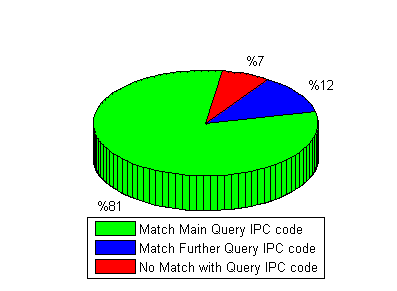
\includegraphics[width=0.50\textwidth,height=55mm]{figs/ipc1stElement.png}
%   \caption{Filter: Only the first component (Section).}   
%   \label{fig:ipc1stElements} 
%\end{figure}
%%%%%%%%%%%%%%%%%%%%%%%%%%%%%%%%%%%%%%%%%%%%%%%%%%%%%%%%%%%%%%%%%%%%%%%%%%%%%%%%%
Figure~\ref{fig:ipc1stElements_a} shows that about 7\% of relevant patents do not share the most general component of the query IPC Code. 
Figure~\ref{fig:ipc1stElements_b} shows the distribution of the number of patents should be ranked for each query after applying the IPC filter.
%: ``\textit{only the first component of the IPC code}". 
The results show that the matching process for each query is done over $ 415828 $ documents, in average, instead of the whole collection (2.6 million documents). This number is much higher than the number for previous filters, which shows that using only the first component of the IPC code is not computationally efficient because it can not reduce the computational time as well as there is still 7\% error. 
%The min number of documents considered during matching process is `$ min=41721 $', and the maximum is `$ max=1058447 $'. 
%\vspace{-2em}
%%%%%%%%%%%%%%%%%%%%%%%%%%%%%%%%%%%%%%%%%%%%%%%%%%%%%%%%%%%%%%%%%%%%%%%%%%%%%%%%%
%\begin{figure}[t!]
%   \centering
%   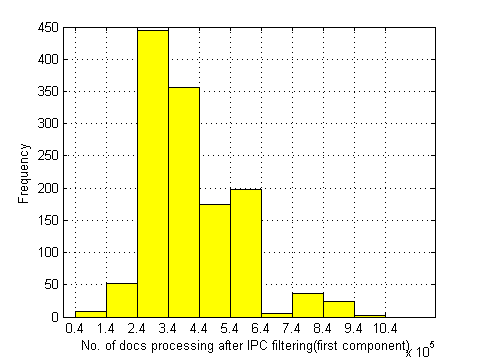
\includegraphics[width=0.60\textwidth,height=60mm]{figs/firstIpcFilter-histo.png}
%   \caption{The distribution of the number of patents should be ranked for a query over all test queries (1303), after applying the IPC filter: ``\textit{only the first component of the IPC code}".
%In average, the matching process for each query is done over `$ 415828 $' documents instead of the whole collection (2.6 million documents). This number is much higher than using more restricted filters and will not be efficient computationally. 
%%The min number of documents considered during matching process is `$ min=41721 $', and the maximum is `$ max=1058447 $'
%}   
%   \label{fig:firstIpcFilter-histo} 
%\end{figure}
%%%%%%%%%%%%%%%%%%%%%%%%%%%%%%%%%%%%%%%%%%%%%%%%%%%%%%%%%%%%%%%%%%%%%%%%%%%%%%%%%

To recap our experiments related to IPC code filtering, we showed that, in trade off between the errors related to applying IPC code filter and computationally efficient matching process, we got the best results when we applied the first three IPC code (Section, Class, and Subclass) of the reference query as a filter. The filter reduced the number of documents to be ranked from the whole collection to $ 36254 $ documents in average, so using IPC filter saved considerable amount of computational time for us.

